\documentclass[a4paper]{article}
\usepackage[utf8x]{inputenc}
\usepackage[danish]{babel}
\usepackage{utopia}
\usepackage{graphicx}
\usepackage{listings}
\usepackage{graphicx}
\usepackage{cmap}

\title{Heaps - ADS}
\author{Edi Begovic | Høgni Jacobsen | Gergö Koncz}
\date{\today}

\def\arraystretch{1.5}
\def\headline#1{\hbox to \hsize{\hrulefill\quad\lower.3em\hbox{#1}\quad\hrulefill}}

\begin{document} 
\maketitle

\ \\
\noindent
The pseudo-code will reference the queue on which the function is called as \textit{q}.
\ \\
\section*{Question 1}
Assuming we wish to draw the resulting binary tree of a max heap:
\ \\
\begin{center}
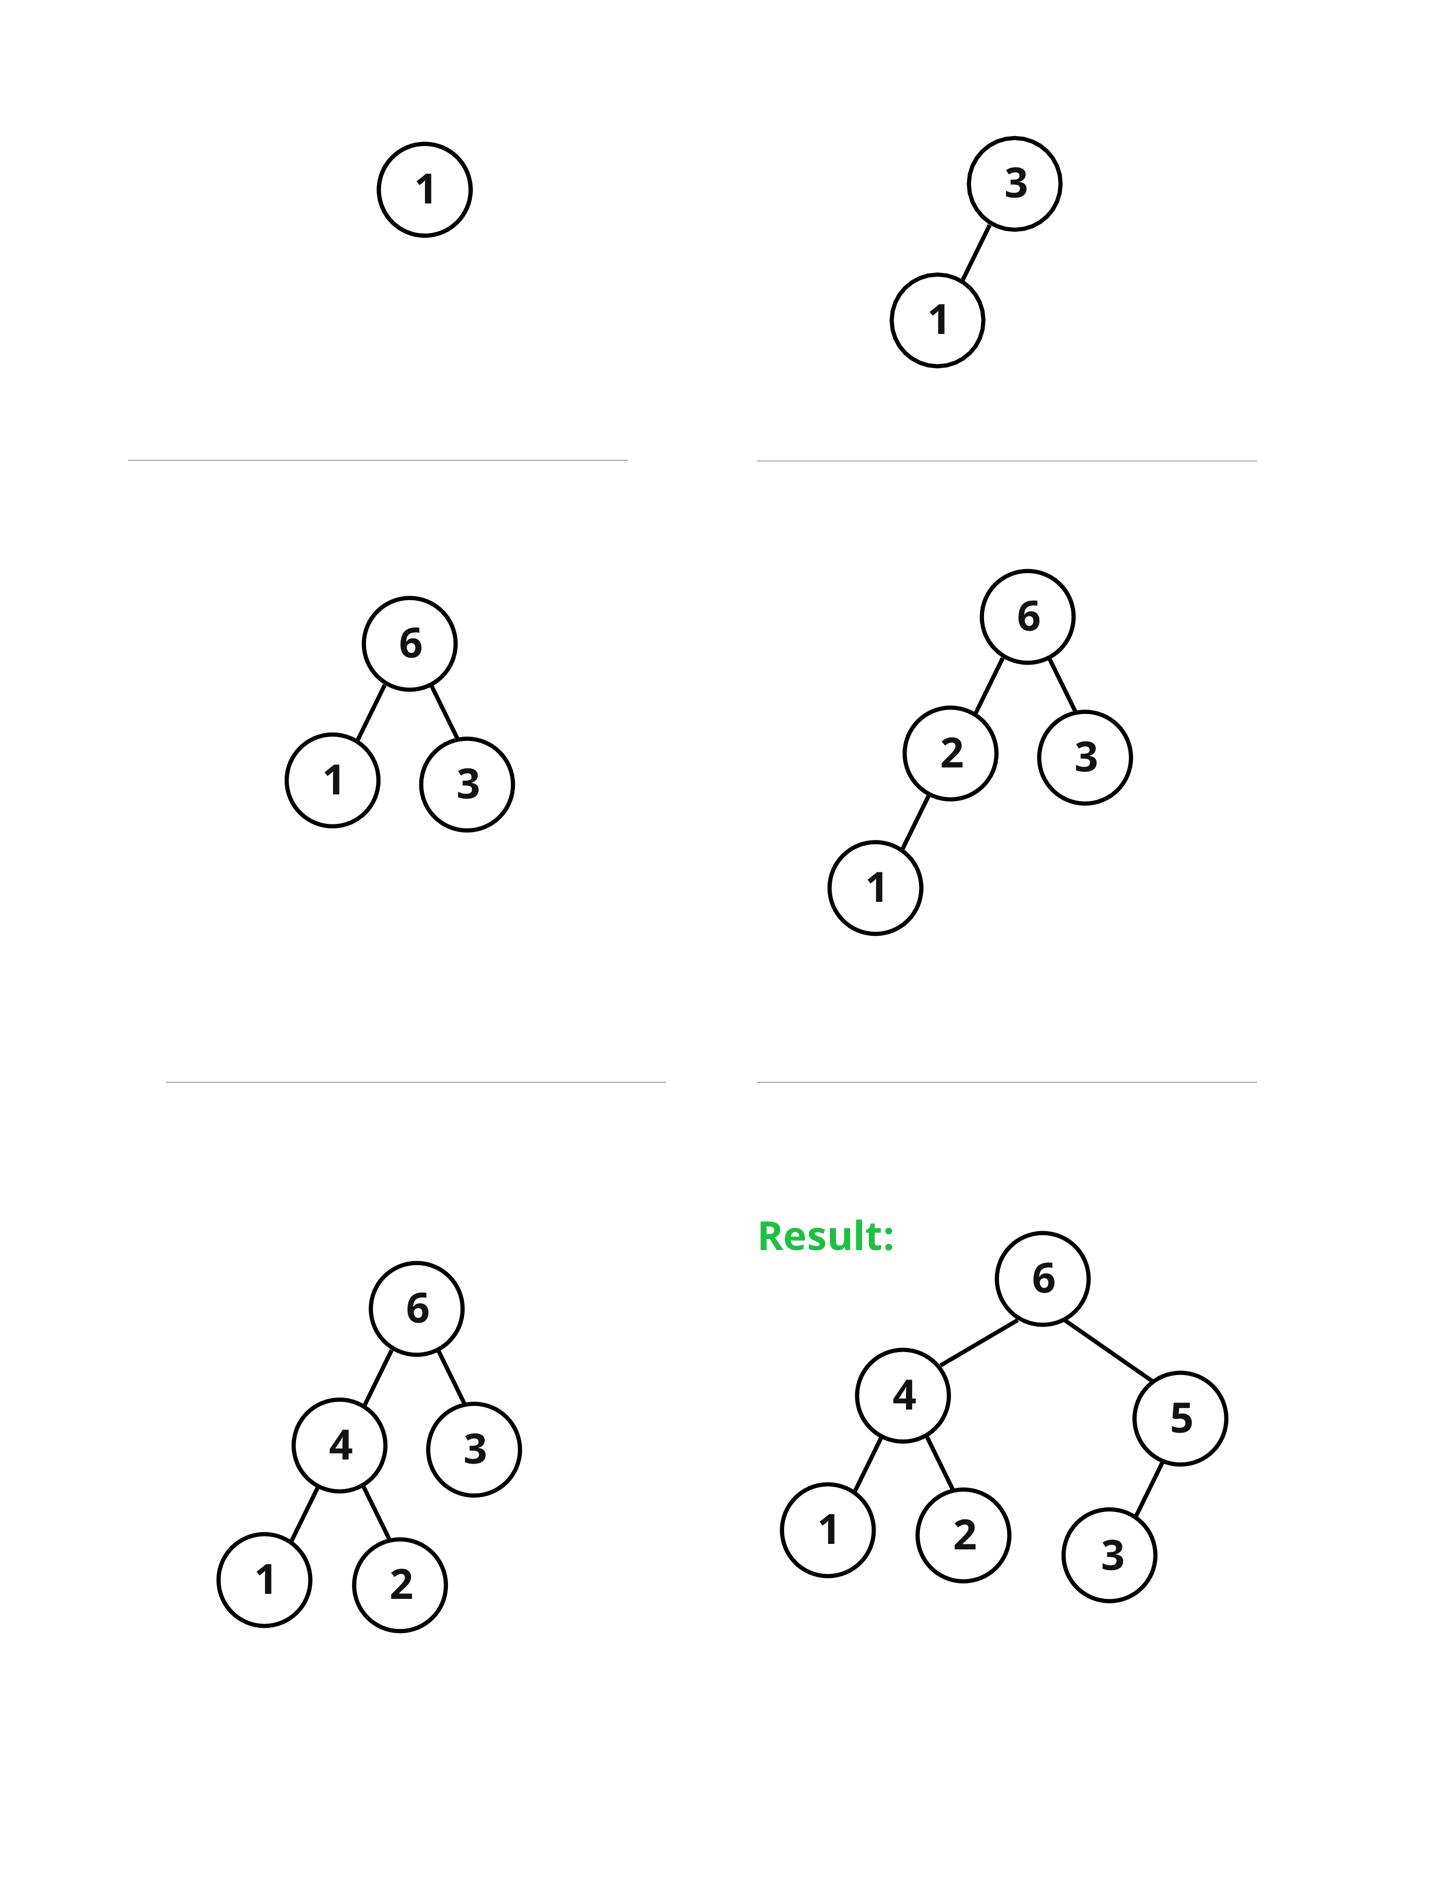
\includegraphics[scale=0.16]{figure1.png}
\end{center}

\noindent
This results in the following array representation: 
$[6, 4, 5, 1, 2, 3]$


\ \\
\section*{Question 2}
\headline{a} \ \\

\noindent
Assuming the 'first' implies the pointer to the first element in the list 
(\textit{that is}, that last added item (p. 148)), answer \textbf{a} is correct.
\ \\

\begin{center}
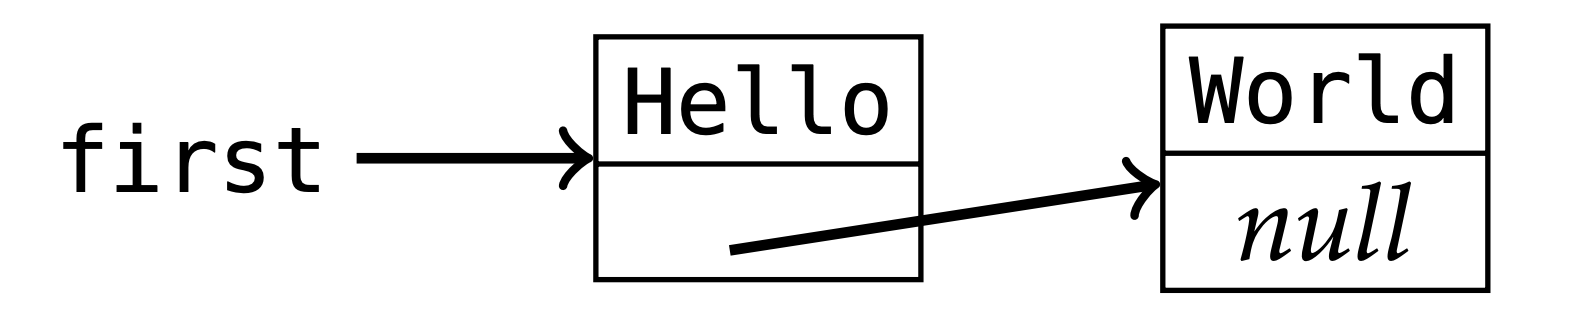
\includegraphics[scale=0.22]{figure2.png}
\end{center}

\headline{b} \ \\

\noindent
The representation of the elements to be unionised have to be the same after the union and since there are already two elements with the number two as their representation it is quicker to change the representation of four to two.\\
\begin{center}
\begin{tabular}{|l|l|l|l|l|}
\hline
\textbf{0} & \textbf{1} & \textbf{2} & \textbf{3} & \textbf{4}\\ 
\hline
0 & 1 & 2 & 2 & 2\\
\hline
\end{tabular}
\end{center}
\ \\

\headline{c} \ \\

\noindent
\textbf{Correct answer:} \\
1. The union operation is asymptotically faster, \textit{as the union operation is now bound by the tree tree height rather than
$N$}.



\ \\

\section*{Question 3}

\noindent
To implement the $min()$ function we cannot just always return the element with 
the last index of the array, since we cannot be certain that the elements at the 
same level are sorted. Also, we cannot iterate through the last level of the tree 
because that would take more than constant time, could be really long by bigger arrays.  
The implementation of a $min()$ function in constant time and space can be 
achieved by keeping track of the minimum element through a variable. We declare it when 
the first element is created, and once a new item is inserted, the new item will be 
compared with the current minimum and replaced if it is lesser than it.


\section*{Question 4}

\noindent
All \textit{hints} were used :) 
\ \\

\noindent
This data structure can be achieved by maintaining two heaps of equal sizes; one max-heap and one min-heap.\ \\

\noindent
As we add items into our data structure, we determine which heap the item belongs to by comparing the root-values
of the two heaps (taking constant time) and adding it to the corresponding heap and \textit{swim} it (taking $log~n$ time).\ \\

\noindent
Should the heap we're adding the item to become larger than the other heap (by more than one item), we simply remove the root 
of this heap and add it to the other. \ \\

\noindent
We thus have a data structure where the root of the largest heap always represents the median value, and should both heaps 
be of the same size, we can simply return the average value of the two roots. 

\end{document} 